\documentclass[aspectratio=169,10pt]{beamer}

\usetheme{Madrid}
\usecolortheme{seahorse}

\usepackage{amsmath,amssymb}
\usepackage{booktabs}
\usepackage{array}
\usepackage{graphicx}
\usepackage{listings}
\usepackage{ragged2e}
\usepackage{tabularx}
\usepackage{tikz}
\usepackage{pgfplots}
\usepackage{iftex}
\pgfplotsset{compat=1.18}

\ifPDFTeX
  \pdfmapfile{+cm.map}
  \pdfmapfile{+cmextra.map}
  \pdfmapfile{+symbols.map}
\fi

\definecolor{CourseBlue}{RGB}{41,77,115}
\definecolor{CourseGreen}{RGB}{63,125,88}
\definecolor{CourseGold}{RGB}{190,137,45}
\definecolor{CourseRed}{RGB}{169,75,70}
\definecolor{SoftGrid}{RGB}{218,225,232}
\definecolor{CodeBack}{RGB}{245,247,249}

\setbeamercolor{structure}{fg=CourseBlue}
\setbeamertemplate{navigation symbols}{}
\setbeamertemplate{itemize items}[circle]
\setbeamertemplate{enumerate items}[default]

\lstdefinestyle{Rstyle}{
  language=R,
  basicstyle=\ttfamily\scriptsize,
  keywordstyle=\color{CourseBlue}\bfseries,
  commentstyle=\color{CourseGreen!80!black},
  stringstyle=\color{CourseRed!85!black},
  backgroundcolor=\color{CodeBack},
  frame=single,
  rulecolor=\color{SoftGrid},
  showstringspaces=false,
  breaklines=true,
  columns=fullflexible,
  keepspaces=true
}

\newcommand{\R}{\mathbb{R}}

\title[Chapter 17: Inference about a Mean]{\textbf{Chapter 17: Inference about a Population Mean}}
\subtitle{The Practice of Statistics in the Life Sciences \\ Brigitte Baldi and David S. Moore}
\author{Instructor: Ali Raisolsadat}
\date{Part IV: Specific Inference Procedures}

\begin{document}

% =============================================================
% INTRODUCTION
% =============================================================

% SLIDE 1
\begin{frame}
  \titlepage
\end{frame}

% SLIDE 2
\begin{frame}{Why Chapter 17 Matters}
Chapter 14 introduced confidence intervals and hypothesis tests for a population mean when the population standard deviation $\sigma$ was known.

\vspace{0.25cm}
In practice, $\sigma$ is rarely known. Chapter 17 replaces it with the sample standard deviation $s$ and develops procedures based on the $t$ distributions.

\begin{block}{Main Question}
How can a sample be used to estimate or test a population mean when both $\mu$ and $\sigma$ are unknown?
\end{block}

The interpretation of confidence intervals and $P$-values remains the same. The probability model used for the calculations changes.
\end{frame}

% SLIDE 3
\begin{frame}{Chapter Roadmap}
The chapter develops six connected ideas.

\begin{enumerate}
  \item Conditions for inference about a population mean
  \item The standard error of a sample mean
  \item The family of $t$ distributions
  \item One-sample $t$ confidence intervals and tests
  \item Matched pairs $t$ procedures
  \item Robustness when the population is not exactly Normal
\end{enumerate}

\vspace{0.2cm}
The theory comes first. Each procedure is then applied to a life-science example and reproduced in R.
\end{frame}

% SLIDE 4
\begin{frame}{Known and Unknown Population Variation}
The difference between the procedures in Chapters 14 and 17 concerns the population standard deviation.

\begin{center}
\begin{tabularx}{0.92\textwidth}{>{\RaggedRight\arraybackslash}p{0.22\textwidth} X X}
\toprule
 & \textbf{Known $\sigma$} & \textbf{Unknown $\sigma$} \\
\midrule
Standard error & $\displaystyle \frac{\sigma}{\sqrt{n}}$ & $\displaystyle \frac{s}{\sqrt{n}}$ \\
Standardized statistic & $z$ & $t$ \\
Reference distribution & Standard Normal & $t$ with $n-1$ degrees of freedom \\
Typical use & Introductory model & Most applications \\
\bottomrule
\end{tabularx}
\end{center}

Estimating $\sigma$ adds uncertainty. The heavier tails of the $t$ distribution account for that extra uncertainty.
\end{frame}

% SLIDE 5
\begin{frame}{The Inference Process}
A one-sample analysis should keep the calculation connected to the research question.

\begin{enumerate}
  \item \textbf{State:} Identify the population and the population mean $\mu$
  \item \textbf{Plan:} Select a one-sample or matched pairs $t$ procedure
  \item \textbf{Solve:} Check the design and distributional conditions, then calculate
  \item \textbf{Conclude:} Interpret the interval or test in the study context
\end{enumerate}

\begin{block}{Design Before Formula}
A correct $t$ calculation cannot remove bias from an inappropriate sample or support a causal conclusion that the study design does not justify.
\end{block}
\end{frame}

% =============================================================
% CONDITIONS AND STANDARD ERROR
% =============================================================

\section{Conditions for Inference}

% SLIDE 6
\begin{frame}{Conditions for Inference about a Mean}
One-sample $t$ procedures rely on two main conditions.

\begin{itemize}
  \item \textbf{Randomness and independence:} The observations can be treated as a simple random sample from a much larger population, or as outcomes from another defensible random process
  \item \textbf{Shape:} The population distribution is Normal, or the sample is large enough for the sampling distribution of $\bar{x}$ to be approximately Normal
\end{itemize}

\vspace{0.25cm}
The random-sampling condition determines whether the sample can represent the target population. The shape condition determines whether the $t$ distribution gives reliable critical values and $P$-values.
\end{frame}

% SLIDE 7
\begin{frame}{Random Sampling and Independence}
The sample should represent the population named in the conclusion.

\begin{itemize}
  \item A simple random sample gives every possible sample of size $n$ an equal chance of selection
  \item If sampling occurs without replacement, the population should be much larger than the sample
  \item A common guideline is $n\leq 0.10N$, where $N$ is the population size
  \item Repeated measurements from the same individual are not independent observations
\end{itemize}

\begin{block}{Scope of Inference}
When a convenience sample is used, calculations may still summarize the observed data, but generalization to a broader population requires caution.
\end{block}
\end{frame}

% SLIDE 8
\begin{frame}{Normality and Sample Size}
The $t$ procedures are exact when the population distribution is Normal. They are often approximately reliable for non-Normal populations when the sample is sufficiently large.

\begin{itemize}
  \item With a small sample, inspect the data for skewness and outliers
  \item As $n$ increases, the Central Limit Theorem improves the Normal approximation for $\bar{x}$
  \item Outliers remain important because both $\bar{x}$ and $s$ are sensitive to extreme values
  \item A large sample does not make a poorly defined population or biased sample appropriate
\end{itemize}

Always examine a graph of the observations before applying a $t$ procedure.
\end{frame}

% SLIDE 9
\begin{frame}{Standard Deviation and Standard Error}
These quantities describe different kinds of variation.

\begin{center}
\begin{tabularx}{0.92\textwidth}{>{\RaggedRight\arraybackslash}p{0.25\textwidth} X X}
\toprule
\textbf{Quantity} & \textbf{Formula} & \textbf{What it describes} \\
\midrule
Sample standard deviation & $s$ & Variation among individual observations in one sample \\
Standard error of $\bar{x}$ & $\displaystyle SE_{\bar{x}}=\frac{s}{\sqrt{n}}$ & Estimated variation among sample means from repeated samples of size $n$ \\
\bottomrule
\end{tabularx}
\end{center}

The standard error describes the precision of the sample mean as an estimate of $\mu$.
\end{frame}

% SLIDE 10
\begin{frame}{The Standard Error of the Mean}
When $\sigma$ is unknown, the sample standard deviation estimates it.

\[
\sigma_{\bar{x}}=\frac{\sigma}{\sqrt{n}}
\qquad\longrightarrow\qquad
SE_{\bar{x}}=\frac{s}{\sqrt{n}}
\]

\begin{itemize}
  \item A smaller $s$ produces a smaller standard error
  \item A larger $n$ produces a smaller standard error
  \item Multiplying $n$ by $4$ divides the standard error by $2$
  \item The value of $s$ changes from sample to sample, so the estimated standard error also changes
\end{itemize}

This sample-to-sample variation in $s$ is why the Standard Normal distribution no longer gives the correct reference model.
\end{frame}

% SLIDE 11
\begin{frame}{From the $z$ Statistic to the $t$ Statistic}
If $\sigma$ is known, standardization gives

\[
z=\frac{\bar{x}-\mu}{\sigma/\sqrt{n}}
\]

If $\sigma$ is unknown, replace it with $s$:

\[
t=\frac{\bar{x}-\mu}{s/\sqrt{n}}
\]

Both statistics measure the distance between the sample mean and a population value in standard-error units. The $t$ statistic has more variability because its denominator is estimated from the same sample.
\end{frame}

% =============================================================
% THE t DISTRIBUTIONS
% =============================================================

\section{The $t$ Distributions}

% SLIDE 12
\begin{frame}{The One-Sample $t$ Statistic}
Suppose a simple random sample of size $n$ comes from a Normal population with unknown mean $\mu$ and unknown standard deviation $\sigma$.

\begin{block}{One-Sample $t$ Statistic}
\[
t=\frac{\bar{x}-\mu}{s/\sqrt{n}}
\]
This statistic follows a $t$ distribution with
\[
df=n-1
\]
degrees of freedom.
\end{block}

The statistic tells us how many estimated standard errors the sample mean lies above or below $\mu$.
\end{frame}

% SLIDE 13
\begin{frame}{Why a New Distribution Is Needed}
The Standard Normal model treats the denominator $\sigma/\sqrt{n}$ as fixed.

\vspace{0.2cm}
The $t$ statistic uses $s/\sqrt{n}$. Because $s$ changes from sample to sample, the standardized statistic varies more than a $z$ statistic.

\begin{block}{Effect on Inference}
The $t$ distributions place more probability in the tails than the Standard Normal distribution. Confidence intervals are therefore wider, and a given standardized distance produces a larger $P$-value.
\end{block}

As the sample size increases, $s$ estimates $\sigma$ more accurately and the difference between $t$ and $z$ becomes smaller.
\end{frame}

% SLIDE 14
\begin{frame}{The Family of $t$ Distributions}
\begin{center}
\begin{tikzpicture}
\begin{axis}[
  width=0.86\textwidth,
  height=0.56\textheight,
  axis lines=left,
  xmin=-4,xmax=4,
  ymin=0,ymax=0.43,
  xtick={-4,-3,-2,-1,0,1,2,3,4},
  ytick=\empty,
  xlabel={Standardized value},
  ylabel={Density},
  grid=major,
  grid style={SoftGrid,dotted},
  legend style={at={(0.5,-0.23)},anchor=north,legend columns=4,draw=none,font=\scriptsize}
]
\addplot[CourseRed,dashed,very thick,smooth] coordinates {(-4,0.00013) (-3.5,0.00087) (-3,0.00443) (-2.5,0.01753) (-2,0.05399) (-1.5,0.12952) (-1,0.24197) (-0.5,0.35207) (0,0.39894) (0.5,0.35207) (1,0.24197) (1.5,0.12952) (2,0.05399) (2.5,0.01753) (3,0.00443) (3.5,0.00087) (4,0.00013)};
\addlegendentry{Normal}
\addplot[CourseGold,very thick,smooth] coordinates {(-4,0.00512) (-3.5,0.00924) (-3,0.01729) (-2.5,0.03333) (-2,0.06509) (-1.5,0.12452) (-1,0.21968) (-0.5,0.32792) (0,0.37961) (0.5,0.32792) (1,0.21968) (1.5,0.12452) (2,0.06509) (2.5,0.03333) (3,0.01729) (3.5,0.00924) (4,0.00512)};
\addlegendentry{$t(5)$}
\addplot[CourseGreen,thick,smooth] coordinates {(-4,0.00203) (-3.5,0.00478) (-3,0.01140) (-2.5,0.02694) (-2,0.06115) (-1.5,0.12744) (-1,0.23036) (-0.5,0.33970) (0,0.38911) (0.5,0.33970) (1,0.23036) (1.5,0.12744) (2,0.06115) (2.5,0.02694) (3,0.01140) (3.5,0.00478) (4,0.00203)};
\addlegendentry{$t(10)$}
\addplot[CourseBlue,thick,smooth] coordinates {(-4,0.00082) (-3.5,0.00261) (-3,0.00796) (-2.5,0.02267) (-2,0.05809) (-1.5,0.12863) (-1,0.23605) (-0.5,0.34581) (0,0.39399) (0.5,0.34581) (1,0.23605) (1.5,0.12863) (2,0.05809) (2.5,0.02267) (3,0.00796) (3.5,0.00261) (4,0.00082)};
\addlegendentry{$t(20)$}
\end{axis}
\end{tikzpicture}
\end{center}
\end{frame}

% SLIDE 15
\begin{frame}{Properties of the $t$ Distributions}
Every $t$ density curve is

\begin{itemize}
  \item Symmetric about $0$
  \item Single-peaked and bell-shaped
  \item More spread out than the Standard Normal curve
  \item Identified by its degrees of freedom
\end{itemize}

\vspace{0.2cm}
Smaller degrees of freedom produce heavier tails. As the degrees of freedom increase, the $t$ distribution approaches the Standard Normal distribution.

\[
t(df)\longrightarrow N(0,1)\quad\text{as }df\text{ increases}
\]
\end{frame}

% SLIDE 16
\begin{frame}{Degrees of Freedom}
For one-sample inference about a mean,

\[
df=n-1
\]

The sample deviations from the sample mean must satisfy

\[
\sum_{i=1}^{n}(x_i-\bar{x})=0
\]

After $n-1$ deviations are known, the final deviation is determined by this constraint. The calculation therefore has $n-1$ independent pieces of information available for estimating variation.

\begin{block}{Practical Use}
The degrees of freedom select the appropriate $t$ curve for critical values and tail probabilities.
\end{block}
\end{frame}

% SLIDE 17
\begin{frame}{Normal and $t$ Critical Values}
The heavier tails of a $t$ distribution lead to larger critical values.

\begin{center}
\begin{tabular}{ccc}
\toprule
\textbf{Reference distribution} & \textbf{Degrees of freedom} & \textbf{95\% critical value} \\
\midrule
$t$ & $5$ & $2.571$ \\
$t$ & $10$ & $2.228$ \\
$t$ & $20$ & $2.086$ \\
$t$ & $50$ & $2.009$ \\
Standard Normal & $\infty$ & $1.960$ \\
\bottomrule
\end{tabular}
\end{center}

The difference is most noticeable for small samples. It becomes modest as the degrees of freedom increase.
\end{frame}

% SLIDE 18
\begin{frame}{Student's $t$ and the Guinness Brewery}
William S. Gosset developed the $t$ distribution while working for the Guinness brewery in the early twentieth century.

\vspace{0.2cm}
His work addressed problems with small samples, including the selection of barley and hops. Guinness restricted employees from publishing company research, so Gosset published under the name ``Student.''

\begin{block}{Statistical Importance}
The method accounts for the uncertainty created when a small sample is used to estimate an unknown population standard deviation.
\end{block}

The name \textbf{Student's $t$ distribution} recognizes Gosset's published work.
\end{frame}

% SLIDE 19
\begin{frame}[fragile]{Areas and Critical Values in R}
R uses \texttt{pt()} for cumulative probabilities and \texttt{qt()} for quantiles.

\begin{lstlisting}[style=Rstyle]
# Area to the left of t = -3 under a t distribution with 10 df
pt(q = -3, df = 10)
# [1] 0.006671828

# Point with 0.95 to its left and 0.05 to its right
qt(p = 0.95, df = 10)
# [1] 1.812461
\end{lstlisting}

\begin{itemize}
  \item \texttt{pt()} answers an area question
  \item \texttt{qt()} answers a cutoff question
  \item Both functions require the degrees of freedom
\end{itemize}
\end{frame}

% SLIDE 20
\begin{frame}{Example 17.1: Reading $t$ Probabilities}
For a $t$ distribution with $10$ degrees of freedom:

\begin{itemize}
  \item The area to the left of $t=-3$ is approximately $0.0067$
  \item The point with probability $0.05$ to its right is approximately $1.812$
\end{itemize}

\[
P(T\leq -3)=0.0067
\]

\[
P(T\geq 1.812)=0.05
\]

Because the distribution is symmetric,

\[
P(T\leq-1.812)=P(T\geq1.812)=0.05
\]
\end{frame}

% =============================================================
% ONE-SAMPLE t CONFIDENCE INTERVAL
% =============================================================

\section{The One-Sample $t$ Confidence Interval}

% SLIDE 21
\begin{frame}{The One-Sample $t$ Confidence Interval}
For a random sample of size $n$ from a population with unknown mean $\mu$ and unknown standard deviation $\sigma$, a level $C$ confidence interval is

\begin{block}{Confidence Interval for $\mu$}
\[
\bar{x}\pm t^*\frac{s}{\sqrt{n}}
\]
where $t^*$ is the critical value from the $t(n-1)$ distribution with central area $C$.
\end{block}

The margin of error is

\[
m=t^*\frac{s}{\sqrt{n}}
\]

The interval is exact for a Normal population and approximately valid for sufficiently large random samples from non-Normal populations.
\end{frame}

% SLIDE 22
\begin{frame}{The Four-Step Confidence-Interval Process}
\begin{enumerate}
  \item \textbf{State:} Define the population and the mean $\mu$ to be estimated
  \item \textbf{Plan:} Choose a confidence level and a one-sample $t$ interval
  \item \textbf{Solve:} Check the sampling and shape conditions, then calculate $\bar{x}$, $s$, $SE$, $t^*$ and the interval
  \item \textbf{Conclude:} Interpret the interval for the population named in the study
\end{enumerate}

\begin{block}{Interpretation}
A level $C$ procedure captures the true population mean in proportion $C$ of repeated random samples under the stated conditions.
\end{block}
\end{frame}

% SLIDE 23
\begin{frame}{Example 17.2: Testosterone in Adolescent Males}
A study recorded plasma testosterone concentrations for $25$ obese adolescent males. The measurements are in nanomoles per litre of blood.

\begin{center}
\scriptsize
\begin{tabular}{rrrrrrrrr}
0.30 & 0.24 & 0.19 & 0.17 & 0.18 & 0.23 & 0.24 & 0.06 & 0.15 \\
0.17 & 0.18 & 0.17 & 0.15 & 0.12 & 0.25 & 0.25 & 0.25 & 0.32 \\
0.35 & 0.37 & 0.39 & 0.46 & 0.49 & 0.42 & 0.36 & & \\
\end{tabular}
\end{center}

\begin{block}{Question}
What is a $95\%$ confidence interval for the mean plasma testosterone concentration among obese adolescent males similar to those represented by the study?
\end{block}
\end{frame}

% SLIDE 24
\begin{frame}{Example 17.2: Parameter and Plan}
Let $\mu$ denote the population mean plasma testosterone concentration for obese adolescent males represented by the study.

\vspace{0.2cm}
The study aims to estimate $\mu$, and the population standard deviation is unknown. The planned procedure is therefore a one-sample $t$ confidence interval.

\begin{block}{Important Scope Limitation}
The participants came from a medical centre rather than a simple random sample of all obese adolescent males. The strongest conclusion applies to a population similar to the individuals who participated.
\end{block}
\end{frame}

% SLIDE 25
\begin{frame}{Example 17.2: Distribution of the Data}
\begin{center}
\begin{tikzpicture}
\begin{axis}[
  width=0.88\textwidth,
  height=0.55\textheight,
  axis lines=left,
  xmin=0.03,xmax=0.52,
  ymin=0.75,ymax=1.35,
  xtick={0.05,0.10,0.15,0.20,0.25,0.30,0.35,0.40,0.45,0.50},
  ytick=\empty,
  xlabel={Plasma testosterone concentration (nmol/L)},
  grid=major,
  grid style={SoftGrid,dotted}
]
\addplot[only marks,mark=*,mark size=2.3pt,CourseBlue]
coordinates {(0.06,1.00) (0.12,1.00) (0.15,1.00) (0.15,1.08) (0.17,1.00) (0.17,1.08) (0.17,1.16) (0.18,1.00) (0.18,1.08) (0.19,1.00) (0.23,1.00) (0.24,1.00) (0.24,1.08) (0.25,1.00) (0.25,1.08) (0.25,1.16) (0.30,1.00) (0.32,1.00) (0.35,1.00) (0.36,1.00) (0.37,1.00) (0.39,1.00) (0.42,1.00) (0.46,1.00) (0.49,1.00)};
\end{axis}
\end{tikzpicture}
\end{center}

The dotplot shows no extreme outliers and no severe skewness. A one-sample $t$ interval is reasonable for these $25$ observations.
\end{frame}

% SLIDE 26
\begin{frame}{Example 17.2: Summary Statistics}
The sample statistics are

\[
n=25
\qquad
\bar{x}=0.2584\text{ nmol/L}
\qquad
s=0.1115\text{ nmol/L}
\]

The estimated standard error is

\[
SE_{\bar{x}}=\frac{s}{\sqrt{n}}=\frac{0.1115}{\sqrt{25}}=0.0223\text{ nmol/L}
\]

This standard error estimates how sample means would vary across repeated samples of $25$ comparable participants.
\end{frame}

% SLIDE 27
\begin{frame}{Example 17.2: Critical Value and Margin of Error}
The degrees of freedom are

\[
df=n-1=25-1=24
\]

For a $95\%$ interval, the two tails contain $0.025$ each, so

\[
t^*_{24}=2.064
\]

The margin of error is

\[
m=t^*\frac{s}{\sqrt{n}}
=2.064(0.0223)
\approx0.0460\text{ nmol/L}
\]
\end{frame}

% SLIDE 28
\begin{frame}{Example 17.2: Confidence Interval}
\[
\bar{x}\pm m
=0.2584\pm0.0460
\]

\[
(0.2124,\ 0.3044)\text{ nmol/L}
\]

\begin{block}{Conclusion}
We are $95\%$ confident that the population mean plasma testosterone concentration for obese adolescent males similar to those studied lies between approximately $0.212$ and $0.304$ nmol/L.
\end{block}

The confidence level describes the long-run performance of the interval-producing method.
\end{frame}

% SLIDE 29
\begin{frame}{Example 17.2: Limits of the Interval}
The interval quantifies random sampling uncertainty under the model.

\begin{itemize}
  \item It estimates a population mean, not the concentration of every individual
  \item It does not correct for a nonrepresentative sample, measurement error or confounding
  \item It does not establish that obesity causes lower testosterone levels
  \item Its strongest scope is a population similar to the study participants
\end{itemize}

The statistical conclusion should remain aligned with the observational study design.
\end{frame}

% SLIDE 30
\begin{frame}[fragile]{Example 17.2: Manual Calculation in R}
\begin{lstlisting}[style=Rstyle]
testosterone <- c(
  0.30, 0.24, 0.19, 0.17, 0.18, 0.23, 0.24, 0.06, 0.15,
  0.17, 0.18, 0.17, 0.15, 0.12, 0.25, 0.25, 0.25, 0.32,
  0.35, 0.37, 0.39, 0.46, 0.49, 0.42, 0.36
)
n <- length(testosterone)
x_bar <- mean(testosterone)
s <- sd(testosterone)
se <- s / sqrt(n)
t_star <- qt(0.975, df = n - 1)
margin <- t_star * se
c(lower = x_bar - margin, upper = x_bar + margin)
\end{lstlisting}
\end{frame}

% SLIDE 31
\begin{frame}[fragile]{Example 17.2: Confidence Interval with \texttt{t.test()}}
\begin{lstlisting}[style=Rstyle]
t.test(testosterone, conf.level = 0.95)
\end{lstlisting}

Relevant output:

\begin{verbatim}
95 percent confidence interval:
 0.2123626 0.3044374
sample estimates:
mean of x
   0.2584
\end{verbatim}

The command also reports a test against the default null value $\mu_0=0$. For this example, the confidence interval is the requested result.
\end{frame}

% SLIDE 32
\begin{frame}{What Controls the Width of a $t$ Interval?}
\[
m=t^*\frac{s}{\sqrt{n}}
\]

\begin{itemize}
  \item A higher confidence level increases $t^*$ and widens the interval
  \item Greater sample variability increases $s$ and widens the interval
  \item A larger sample size decreases $s/\sqrt{n}$ and usually narrows the interval
  \item A different sample can change both $\bar{x}$ and $s$
\end{itemize}

Multiplying the sample size by $4$ approximately halves the standard error when the underlying variability remains similar.
\end{frame}

% SLIDE 33
\begin{frame}{Common Confidence-Interval Errors}
\begin{itemize}
  \item Using $z^*=1.960$ when $\sigma$ is unknown and the sample is small
  \item Using $s$ instead of $s/\sqrt{n}$ as the standard error
  \item Forgetting that the procedure uses $df=n-1$
  \item Interpreting the interval as a range for individual observations
  \item Ignoring a severe outlier or a sample-selection problem
\end{itemize}

\begin{block}{Useful Check}
The interval should be centred at $\bar{x}$, and its width should reflect the confidence level, variability and sample size.
\end{block}
\end{frame}

% =============================================================
% ONE-SAMPLE t TEST
% =============================================================

\section{The One-Sample $t$ Test}

% SLIDE 34
\begin{frame}{The One-Sample $t$ Test}
To test a claim about an unknown population mean, begin with

\[
H_0:\mu=\mu_0
\]

The test statistic is

\begin{block}{One-Sample $t$ Statistic}
\[
t=\frac{\bar{x}-\mu_0}{s/\sqrt{n}}
\]
with $df=n-1$.
\end{block}

The statistic measures the distance from the observed sample mean to the null value in estimated standard-error units.
\end{frame}

% SLIDE 35
\begin{frame}{The Alternative Determines the Tail}
Let $T$ follow a $t(n-1)$ distribution under $H_0$.

\begin{center}
\begin{tabularx}{0.88\textwidth}{>{\centering\arraybackslash}p{0.25\textwidth} X}
\toprule
\textbf{Alternative} & \textbf{$P$-value} \\
\midrule
$H_a:\mu>\mu_0$ & $P(T\geq t_{\text{{obs}}})$ \\
$H_a:\mu<\mu_0$ & $P(T\leq t_{\text{{obs}}})$ \\
$H_a:\mu\neq\mu_0$ & $2P(T\geq |t_{\text{{obs}}}|)$ \\
\bottomrule
\end{tabularx}
\end{center}

The direction of the alternative should follow from the research question before the sample result is examined.
\end{frame}

% SLIDE 36
\begin{frame}{The Four-Step Hypothesis-Test Process}
\begin{enumerate}
  \item \textbf{State:} Define $\mu$ and state $H_0$ and $H_a$
  \item \textbf{Plan:} Select a one-sample $t$ test and a significance level if a formal decision is required
  \item \textbf{Solve:} Check conditions, calculate the test statistic and obtain the $P$-value from $t(n-1)$
  \item \textbf{Conclude:} Describe the evidence in context without claiming that $H_0$ has been proved
\end{enumerate}

\begin{block}{Meaning of the $P$-Value}
The $P$-value is calculated under the assumption that $H_0$ and the statistical model are true.
\end{block}
\end{frame}

% SLIDE 37
\begin{frame}{Example 17.3: Pulse Wave Velocity and Progeria}
Pulse wave velocity (PWV) measures vascular stiffness. A study recorded PWV, in metres per second, for $18$ children diagnosed with progeria.

\begin{center}
\small
\begin{tabular}{rrrrrrrrr}
18.8 & 17.6 & 17.5 & 16.0 & 14.8 & 14.1 & 13.7 & 13.1 & 12.9 \\
12.9 & 12.4 & 10.1 & 9.3 & 9.1 & 8.3 & 8.3 & 7.9 & 7.2 \\
\end{tabular}
\end{center}

In healthy children, values greater than $6.6$ m/s would be considered abnormal.

\begin{block}{Question}
Do the data provide evidence that the population mean PWV for children with progeria is greater than $6.6$ m/s?
\end{block}
\end{frame}

% SLIDE 38
\begin{frame}{Example 17.3: Distribution of PWV}
\begin{center}
\begin{tikzpicture}
\begin{axis}[
  width=0.88\textwidth,
  height=0.55\textheight,
  axis lines=left,
  xmin=6.5,xmax=19.5,
  ymin=0.75,ymax=1.30,
  xtick={7,9,11,13,15,17,19},
  ytick=\empty,
  xlabel={Pulse wave velocity (m/s)},
  grid=major,
  grid style={SoftGrid,dotted}
]
\addplot[only marks,mark=*,mark size=2.5pt,CourseRed]
coordinates {(7.2,1.00) (7.9,1.00) (8.3,1.00) (8.3,1.09) (9.1,1.00) (9.3,1.00) (10.1,1.00) (12.4,1.00) (12.9,1.00) (12.9,1.09) (13.1,1.00) (13.7,1.00) (14.1,1.00) (14.8,1.00) (16.0,1.00) (17.5,1.00) (17.6,1.00) (18.8,1.00)};
\end{axis}
\end{tikzpicture}
\end{center}

The sample shows no isolated extreme outlier. With $n=18$ and no severe departure from a single-peaked distribution, a one-sample $t$ test is reasonable.
\end{frame}

% SLIDE 39
\begin{frame}{Example 17.3: Hypotheses}
Let $\mu$ be the population mean PWV for children with progeria represented by the study.

\[
H_0:\mu=6.6\text{ m/s}
\]

\[
H_a:\mu>6.6\text{ m/s}
\]

The alternative is upper-tailed because the research question asks whether the mean PWV is higher than the reference value.

\begin{block}{Study Scope}
Progeria is rare, and the participants were recruited worldwide rather than selected through a formal SRS. The conclusion applies most directly to comparable children with progeria.
\end{block}
\end{frame}

% SLIDE 40
\begin{frame}{Example 17.3: Summary and Standard Error}
The sample statistics are

\[
n=18
\qquad
\bar{x}=12.444\text{ m/s}
\qquad
s=3.638\text{ m/s}
\]

The estimated standard error is

\[
SE_{\bar{x}}=\frac{3.638}{\sqrt{18}}\approx0.857\text{ m/s}
\]

If $H_0$ were true, this standard error would describe the estimated sample-to-sample variability of $\bar{x}$ around $6.6$ m/s.
\end{frame}

% SLIDE 41
\begin{frame}{Example 17.3: Test Statistic}
The degrees of freedom are

\[
df=18-1=17
\]

The test statistic is

\[
t=\frac{\bar{x}-\mu_0}{s/\sqrt{n}}
=\frac{12.444-6.6}{3.638/\sqrt{18}}
\approx6.816
\]

The observed sample mean is approximately $6.82$ estimated standard errors above the null value.
\end{frame}

% SLIDE 42
\begin{frame}{Example 17.3: $P$-Value}
The alternative is $H_a:\mu>6.6$, so the $P$-value is the upper-tail area under the $t(17)$ distribution.

\[
P(T\geq6.816)\approx0.0000015
\]

\begin{block}{Interpretation}
If the population mean were $6.6$ m/s and the model conditions held, a sample mean at least as high as the observed value would occur in approximately $1.5$ out of every million repeated samples of size $18$.
\end{block}

The very small $P$-value provides very strong evidence against $H_0$.
\end{frame}

% SLIDE 43
\begin{frame}{Example 17.3: Conclusion and Effect Size}
The data provide very strong evidence that the population mean PWV for comparable children with progeria is greater than $6.6$ m/s.

\vspace{0.25cm}
The observed difference from the reference value is

\[
12.444-6.6=5.844\text{ m/s}
\]

Statistical significance addresses evidence against the null model. The size and clinical importance of the difference require subject-matter interpretation and should not be judged from the $P$-value alone.
\end{frame}

% SLIDE 44
\begin{frame}[fragile]{Example 17.3: Manual Test in R}
\begin{lstlisting}[style=Rstyle]
pwv <- c(
  18.8, 17.6, 17.5, 16.0, 14.8, 14.1, 13.7, 13.1, 12.9,
  12.9, 12.4, 10.1, 9.3, 9.1, 8.3, 8.3, 7.9, 7.2
)

n <- length(pwv)
x_bar <- mean(pwv)
s <- sd(pwv)
t_stat <- (x_bar - 6.6) / (s / sqrt(n))
p_value <- pt(t_stat, df = n - 1, lower.tail = FALSE)

c(t = t_stat, p_value = p_value)
\end{lstlisting}
\end{frame}

% SLIDE 45
\begin{frame}[fragile]{Example 17.3: Test with \texttt{t.test()}}
\begin{lstlisting}[style=Rstyle]
t.test(
  pwv,
  mu = 6.6,
  alternative = "greater"
)
\end{lstlisting}

Relevant output:

\begin{verbatim}
t = 6.8163, df = 17, p-value = 1.501e-06
alternative hypothesis: true mean is greater than 6.6
sample estimates:
mean of x
 12.44444
\end{verbatim}

The value supplied to \texttt{alternative} must match the stated research hypothesis.
\end{frame}

% SLIDE 46
\begin{frame}{Confidence Intervals and Two-Sided Tests}
When a two-sided test and a confidence interval use the same data, model and significance level,

\begin{itemize}
  \item Reject $H_0:\mu=\mu_0$ at level $\alpha$ if $\mu_0$ lies outside the corresponding $(1-\alpha)100\%$ confidence interval
  \item Fail to reject $H_0$ if $\mu_0$ lies inside the interval
\end{itemize}

\begin{block}{Different Information}
The test evaluates a specific null value. The confidence interval displays a range of plausible population means and communicates the precision of the estimate.
\end{block}
\end{frame}

% =============================================================
% MATCHED PAIRS
% =============================================================

\section{Matched Pairs $t$ Procedures}

% SLIDE 47
\begin{frame}{Why Matched Pairs Are Useful}
Many studies compare two conditions using observations that are naturally connected.

\begin{itemize}
  \item The same individual is measured before and after a treatment
  \item Each participant receives both conditions at different times
  \item Individuals are paired using relevant characteristics before receiving different treatments
\end{itemize}

Matching can reduce variation caused by differences among individuals. The analysis must preserve the pairing created by the study design.
\end{frame}

% SLIDE 48
\begin{frame}{Matched Pairs Become One Sample}
For each pair, calculate one difference.

\[
d_i=\text{response under condition 2}-\text{response under condition 1}
\]

The paired dataset becomes

\[
d_1,d_2,\ldots,d_n
\]

Apply the one-sample $t$ procedures to the differences.

\begin{block}{Parameter}
$\mu_d$ is the population mean of the pairwise differences. A value of $\mu_d=0$ represents no mean change under the chosen subtraction order.
\end{block}
\end{frame}

% SLIDE 49
\begin{frame}{The Direction of the Difference}
The subtraction order determines the sign of the parameter and the alternative hypothesis.

\begin{center}
\begin{tabularx}{0.92\textwidth}{>{\RaggedRight\arraybackslash}p{0.30\textwidth} X X}
\toprule
\textbf{Definition} & \textbf{Improvement means} & \textbf{Alternative} \\
\midrule
$d=\text{after}-\text{before}$ & Negative differences & $H_a:\mu_d<0$ \\
$d=\text{before}-\text{after}$ & Positive differences & $H_a:\mu_d>0$ \\
\bottomrule
\end{tabularx}
\end{center}

Either definition is valid when it is stated clearly and used consistently throughout the calculation and conclusion.
\end{frame}

% SLIDE 50
\begin{frame}{Matched Pairs Conditions}
The one-sample conditions apply to the \textbf{differences}.

\begin{itemize}
  \item The pairs or participants should represent the target population through a defensible sampling process
  \item The pairwise differences should be independent across pairs
  \item The distribution of the differences should be approximately Normal, or the number of pairs should be large enough
  \item Inspect the differences for skewness and outliers
\end{itemize}

The two measurements within a pair are expected to be dependent. That dependence is the reason for pairing them.
\end{frame}

% SLIDE 51
\begin{frame}{Example 17.4: Treatment for Progeria}
The $18$ children in the PWV study received lonafarnib for two years. Researchers measured PWV before and after treatment.

\begin{block}{Question}
Do the paired data provide evidence that the treatment lowers mean PWV among comparable children with progeria?
\end{block}

Define

\[
d=\text{treated PWV}-\text{untreated PWV}
\]

A reduction produces a negative difference. The hypotheses are

\[
H_0:\mu_d=0
\qquad
H_a:\mu_d<0
\]
\end{frame}

% SLIDE 52
\begin{frame}{Example 17.4: Paired Measurements}
\scriptsize
\begin{center}
\begin{tabular}{crrr@{\hspace{0.7cm}}crrr}
\toprule
\textbf{Child} & \textbf{Before} & \textbf{After} & $d$ &
\textbf{Child} & \textbf{Before} & \textbf{After} & $d$ \\
\midrule
1 & 18.8 & 12.6 & $-6.2$ & 10 & 12.9 & 7.5 & $-5.4$ \\
2 & 17.6 & 10.8 & $-6.8$ & 11 & 12.4 & 9.4 & $-3.0$ \\
3 & 17.5 & 10.1 & $-7.4$ & 12 & 10.1 & 6.4 & $-3.7$ \\
4 & 16.0 & 10.1 & $-5.9$ & 13 & 9.3 & 9.0 & $-0.3$ \\
5 & 14.8 & 9.2 & $-5.6$ & 14 & 9.1 & 6.2 & $-2.9$ \\
6 & 14.1 & 7.6 & $-6.5$ & 15 & 8.3 & 7.2 & $-1.1$ \\
7 & 13.7 & 10.8 & $-2.9$ & 16 & 7.9 & 7.3 & $-0.6$ \\
8 & 13.1 & 7.7 & $-5.4$ & 17 & 8.3 & 5.7 & $-2.6$ \\
9 & 12.9 & 6.8 & $-6.1$ & 18 & 7.2 & 9.1 & $1.9$ \\
\bottomrule
\end{tabular}
\end{center}

The measurements are paired by child. The $18$ differences, not the $36$ individual measurements, form the sample for the $t$ analysis.
\end{frame}

% SLIDE 53
\begin{frame}{Example 17.4: Distribution of Differences}
\begin{center}
\begin{tikzpicture}
\begin{axis}[
  width=0.88\textwidth,
  height=0.55\textheight,
  axis lines=left,
  xmin=-8,xmax=3,
  ymin=0.75,ymax=1.30,
  xtick={-8,-6,-4,-2,0,2},
  ytick=\empty,
  xlabel={Treated PWV $-$ untreated PWV (m/s)},
  grid=major,
  grid style={SoftGrid,dotted}
]
\addplot[only marks,mark=*,mark size=2.5pt,CourseGreen]
coordinates {(-7.4,1.00) (-6.8,1.00) (-6.5,1.00) (-6.2,1.00) (-6.1,1.00) (-5.9,1.00) (-5.6,1.00) (-5.4,1.00) (-5.4,1.09) (-3.7,1.00) (-3.0,1.00) (-2.9,1.00) (-2.9,1.09) (-2.6,1.00) (-1.1,1.00) (-0.6,1.00) (-0.3,1.00) (1.9,1.00)};
\addplot[CourseRed,dashed,thick] coordinates {(0,0.82) (0,1.23)};
\end{axis}
\end{tikzpicture}
\end{center}

The distribution shows mild skewness and no isolated extreme outlier. A paired $t$ procedure is reasonable for the $18$ differences.
\end{frame}

% SLIDE 54
\begin{frame}{Example 17.4: Summary Statistics}
For the $18$ differences,

\[
n=18
\qquad
\bar{d}=-3.917\text{ m/s}
\qquad
s_d=2.644\text{ m/s}
\]

The standard error is

\[
SE_{\bar{d}}=\frac{s_d}{\sqrt{n}}
=\frac{2.644}{\sqrt{18}}
\approx0.623\text{ m/s}
\]

The negative sample mean indicates that PWV was lower after treatment, on average, in the observed sample.
\end{frame}

% SLIDE 55
\begin{frame}{Example 17.4: Test Statistic and $P$-Value}
The test statistic is

\[
t=\frac{\bar{d}-0}{s_d/\sqrt{n}}
=\frac{-3.917}{2.644/\sqrt{18}}
\approx-6.286
\]

with $df=17$. Because $H_a:\mu_d<0$, the $P$-value is the lower-tail area.

\[
P(T\leq-6.286)\approx0.0000041
\]

The paired data provide very strong evidence that the treatment lowers mean PWV for comparable children with progeria.
\end{frame}

% SLIDE 56
\begin{frame}{Example 17.4: Confidence Interval for Mean Change}
A $95\%$ interval for the mean difference is

\[
\bar{d}\pm t^*\frac{s_d}{\sqrt{n}}
\]

\[
-3.917\pm2.110(0.623)
\]

\[
(-5.231,\ -2.602)\text{ m/s}
\]

Using $d=\text{after}-\text{before}$, the interval is negative. Equivalently, the estimated population mean reduction is between approximately $2.60$ and $5.23$ m/s.
\end{frame}

% SLIDE 57
\begin{frame}{Statistical and Clinical Importance}
The very small $P$-value provides strong evidence of a mean reduction in PWV. The confidence interval estimates the size of that reduction.

\vspace{0.25cm}
Neither result determines whether the reduction is clinically important. That judgment requires knowledge of

\begin{itemize}
  \item How a change in PWV relates to health outcomes
  \item The treatment's side effects and burdens
  \item The variation in responses among individual patients
\end{itemize}

Statistical evidence should be combined with clinical expertise and the full study design.
\end{frame}

% SLIDE 58
\begin{frame}[fragile]{Example 17.4: Paired Test in R}
\begin{lstlisting}[style=Rstyle]
before <- c(
  18.8, 17.6, 17.5, 16.0, 14.8, 14.1, 13.7, 13.1, 12.9,
  12.9, 12.4, 10.1, 9.3, 9.1, 8.3, 7.9, 8.3, 7.2
)
after <- c(
  12.6, 10.8, 10.1, 10.1, 9.2, 7.6, 10.8, 7.7, 6.8,
  7.5, 9.4, 6.4, 9.0, 6.2, 7.2, 7.3, 5.7, 9.1
)

t.test(after, before, paired = TRUE, alternative = "less")
\end{lstlisting}

R forms \texttt{after - before}, matching the stated definition of the differences.
\end{frame}

% SLIDE 59
\begin{frame}{Why the Pairing Must Be Preserved}
Treating the before and after measurements as two independent samples would ignore the connection between observations from the same child.

\begin{itemize}
  \item The independent-samples model assumes that the two groups do not share observational units
  \item The matched pairs model uses each child as their own comparison
  \item The variation among children is partly removed by working with within-child differences
\end{itemize}

\begin{block}{General Principle}
The inferential procedure must reflect the design that produced the data.
\end{block}
\end{frame}

% =============================================================
% ROBUSTNESS
% =============================================================

\section{Robustness of $t$ Procedures}

% SLIDE 60
\begin{frame}{Robust Statistical Procedures}
A procedure is \textbf{robust} when moderate violations of its conditions have little effect on the reported confidence level or $P$-value.

\vspace{0.25cm}
One-sample $t$ procedures are reasonably robust to non-Normal population shapes when the sample is large enough.

\begin{block}{Important Exception}
The procedures are sensitive to outliers because both $\bar{x}$ and $s$ can change substantially when one extreme observation is present.
\end{block}

Robustness to distribution shape does not correct selection bias, dependence or measurement problems.
\end{frame}

% SLIDE 61
\begin{frame}{Practical Sample-Size Guidelines}
\begin{center}
\begin{tabularx}{0.94\textwidth}{>{\RaggedRight\arraybackslash}p{0.22\textwidth} X}
\toprule
\textbf{Sample size} & \textbf{Practical guidance} \\
\midrule
$n<15$ & Use $t$ procedures when the data are roughly symmetric and single-peaked, with no outliers \\
$15\leq n<40$ & Mild skewness is usually acceptable, but strong skewness or outliers remain concerning \\
$n\geq40$ & Strong skewness is often manageable, although influential outliers still require investigation \\
\bottomrule
\end{tabularx}
\end{center}

These are guidelines rather than automatic rules. The data-collection design remains more important than the exact population shape.
\end{frame}

% SLIDE 62
\begin{frame}{A Practical Screening Process}
Before using a one-sample or matched pairs $t$ procedure:

\begin{enumerate}
  \item Identify the observational units and the target population
  \item Confirm whether the observations or pairwise differences can be treated as independent
  \item Plot the observations or differences
  \item Look for isolated outliers, strong skewness and multiple groups
  \item Consider the sample size together with the observed shape
  \item Investigate unusual values before removing or altering them
\end{enumerate}

The graph and study design determine whether the numerical procedure answers a meaningful question.
\end{frame}

% SLIDE 63
\begin{frame}{Example 17.5: Small and Moderate Samples}
\begin{center}
\begin{tabularx}{0.94\textwidth}{>{\RaggedRight\arraybackslash}p{0.25\textwidth} >{\centering\arraybackslash}p{0.12\textwidth} X}
\toprule
\textbf{Dataset} & \textbf{Size} & \textbf{Assessment} \\
\midrule
Oak acorn volumes & $n=11$ & One clear, extreme outlier makes $t$ procedures unreliable for this small sample \\
Aleppo pine needle lengths & $n=15$ & Mild right skewness with no outliers is acceptable for a moderate sample \\
\bottomrule
\end{tabularx}
\end{center}

The difference between the examples is not only the sample size. The extreme outlier in the acorn data directly affects both the sample mean and sample standard deviation.
\end{frame}

% SLIDE 64
\begin{frame}{Example 17.5: Large Samples}
\begin{center}
\begin{tabularx}{0.94\textwidth}{>{\RaggedRight\arraybackslash}p{0.25\textwidth} >{\centering\arraybackslash}p{0.12\textwidth} X}
\toprule
\textbf{Dataset} & \textbf{Size} & \textbf{Assessment} \\
\midrule
Brown treesnake weights & About $500$ & Strong right skewness is manageable at this size, but the heaviest snake should still be investigated for influence \\
Wild bee cocoon widths & About $800$ & Computation is stable, but the clear bimodality makes one overall mean scientifically difficult to interpret \\
\bottomrule
\end{tabularx}
\end{center}

A large sample can improve the sampling distribution of $\bar{x}$. It cannot make a scientifically unhelpful summary meaningful.
\end{frame}

% SLIDE 65
\begin{frame}{Bimodality and the Meaning of a Mean}
The wild bee cocoon distribution contains two groups because female and male cocoons differ in width.

\vspace{0.2cm}
An overall mean combines

\begin{itemize}
  \item The mean width within each biological group
  \item The proportion of observations belonging to each group
\end{itemize}

If the sex composition changes, the overall mean can change even when neither group changes.

\begin{block}{Analysis Choice}
Separate summaries or a model that includes sex may answer the biological question more clearly than one confidence interval for a pooled mean.
\end{block}
\end{frame}

% SLIDE 66
\begin{frame}{When an Outlier Appears}
An unusual observation should be examined rather than deleted automatically.

\begin{itemize}
  \item Check for data-entry, unit or measurement errors
  \item Confirm whether the observation belongs to the target population
  \item Compare the analysis with and without the observation as a sensitivity check
  \item Report any decision to exclude an observation and explain the reason
  \item Consider a transformation or another method when the population is strongly skewed
\end{itemize}

An outlier may be an error, a valid rare value or evidence that the population contains distinct subgroups.
\end{frame}

% SLIDE 67
\begin{frame}{Choosing the Correct Procedure}
\begin{center}
\begin{tabularx}{0.94\textwidth}{>{\RaggedRight\arraybackslash}p{0.30\textwidth} X}
\toprule
\textbf{Study structure} & \textbf{Procedure} \\
\midrule
One quantitative sample, unknown $\sigma$ & One-sample $t$ interval or test \\
Two measurements on each individual & Paired $t$ procedure applied to within-individual differences \\
Legitimately matched pairs & Paired $t$ procedure applied to within-pair differences \\
Two separate, unrelated groups & Independent two-sample procedure, studied in the next chapter \\
\bottomrule
\end{tabularx}
\end{center}

The number of columns in a dataset does not determine the method. The design and dependence structure do.
\end{frame}

% SLIDE 68
\begin{frame}{Chapter 17 Summary}
\begin{itemize}
  \item When $\sigma$ is unknown, estimate the standard error of $\bar{x}$ with $s/\sqrt{n}$
  \item Use the $t(n-1)$ distribution for one-sample confidence intervals and tests
  \item A level $C$ confidence interval is $\bar{x}\pm t^*s/\sqrt{n}$
  \item A test of $H_0:\mu=\mu_0$ uses $t=(\bar{x}-\mu_0)/(s/\sqrt{n})$
  \item Matched pairs procedures apply one-sample $t$ methods to pairwise differences
  \item Inspect the data and study design before relying on the procedure
\end{itemize}

\begin{block}{Final Principle}
The calculation quantifies sampling uncertainty. The design, data quality and scientific context determine what the result can mean.
\end{block}
\end{frame}

\end{document}




